\documentclass[a4paper,10pt]{book}
\usepackage[centertags]{amsmath}
\usepackage{amscd}
\usepackage{amsthm}
\usepackage{amssymb}
\usepackage{enumerate}
\usepackage{multicol}
\usepackage[english,catalan,spanish]{babel}
\usepackage[all]{xy}
\usepackage{color}
\usepackage{tikz}
\usepackage{indentfirst}
\usepackage[utf8]{inputenc}
\usepackage[T1]{fontenc}
\linespread{1.1}
\setlength{\parskip}{10pt}
\usepackage[twoside,bindingoffset=1cm]{geometry}
\usepackage{lmodern}
\usepackage[x11names, dvipsnames, table]{xcolor}
\definecolor{ubblue}{HTML}{0059A2}
\usepackage[colorlinks=true, linkcolor=black, citecolor=ubblue, urlcolor=ubblue]{hyperref}
\usepackage{cleveref}
\usepackage[protrusion=true,expansion=true]{microtype}
\usepackage{cite}
\usepackage{booktabs}
\usepackage{IEEEtrantools}
\usepackage{subcaption}
\usepackage{enumitem}
\setlist[itemize]{itemsep=4pt, parsep=2pt, topsep=2pt, leftmargin=*}




%% Custom packages


%%%%%%%%%%%%%%%%%%%%%%%%%%%%%%%%%%%%%%%%%%%%%%%%%%%%%%%%%%%%%%%%%%%%%%%%%%%
%%%% local definitions for this paper
%%%%%%%%%%%%%%%%%%%%%%%%%%%%%%%%%%%%%%%%%%%%%%%%%%%%%%%%%%%%%%%%%%%%%%%%%%%


%%%%%%%%%%%%%%%%%%%%%% aix{\`o} pels headings %%%%%%%%%%%%%%%%%%%%%%%%
\usepackage{fancyhdr}
\setlength{\headheight}{12.69002pt}
\pagestyle{fancy}
\renewcommand{\chaptermark}[1]{\markboth{#1}{}}
\renewcommand{\sectionmark}[1]{\markright{\thesection\ #1}}
\fancyhf{} \fancyhead[LE,RO]{\bfseries\thepage}
\fancyhead[LO]{\bfseries\rightmark} \fancyhead[RE]{\bfseries\leftmark}

\def\paginaenblanc{\newpage%
\thispagestyle{empty}%
\vspace*{2cm}%
\newpage%
\thispagestyle{empty}%
}


%%%%%%%%%%%%%%%%%%%%%%%%%%%%%%%%%%%%%%%%%%%%%%%%%%%%%%%%%%%%%%%%%%%%%%%%%
% aux commands
%%%%%%%%%%%%%%%%%%%%%%%%%%%%%%%%%%%%%%%%%%%%%%%%%%%%%%%%%%%%%%%%%%%%%%%%%
%==========================================================================
% macros to support private authors' notes
%==========================================================================
\newif\ifprivate
\privatetrue
\def\xbar{\vskip0.09in\hrule\vskip0.06in}
\def\private#1{\ifprivate \xbar {\em #1} \xbar
\else \fi}
\def\huh{\ifprivate ??? \marginpar{\Huge ???}
\else \fi}
\def\???{\ifprivate {\bf {???}} \marginpar{\begin{center}{\Huge {\bf ?}}\end{center}}
\else \fi}
%\def\???{\ifprivate {\bf {???}} \marginpar{{\Huge {\bf ?}}}
%\else \fi}
\marginparsep1mm
\def\nota#1{\ifprivate  $\clubsuit$ \marginpar{\parbox[t]{2.4cm}{\begin{center}\tiny #1\end{center}}}
\else \fi}
\def\comment#1{\ifprivate \marginpar{\parbox[t]{2.4cm}{\begin{center}\tiny #1\end{center}}}
\else \fi}
%\def\nota#1{\ifprivate  $\clubsuit$ \marginpar{\parbox[t]{1.8cm}{\tiny #1}}
%\else \fi}
\def\privateeject{\ifprivate\eject\fi}
%\def\???{{\bf {???}} \marginpar{{\Huge {\bf ?}}} }
%%%%%%%%%%%%%%%%%%%%%%%%%%%%%%%%%%%%%%%%%%%%%%%%%%%%%%%%%%%%%%%%%%%%%%%%%%

%%%%%%%%%%%%%%%%%%%%%%%%%%%%%%%%%%%%%%%%%%%%%%%%%%%%%%%%%%%%%%%%%%%%%%%%
%%%%%%%%%%%%%%%%%%%%%%%%%%%%%%%%%%%%%%%%%%%%%%%%%%%%%%%%%%%%%%%%%%%%%%%%
\begin{document}
\bstctlcite{IEEEexample:BSTcontrol}
\pagestyle{empty}

\begin{titlepage}
	\begin{center}
		\begin{figure}[htb]
			\begin{center}
				
\includegraphics[width=6cm]{assets/ub_color.pdf}
			\end{center}
		\end{figure}
		
		\def\worktitle{Development of an AI-Based Tool for Molecular Subtype Classification of Invasive Ductal Breast Carcinoma Using Mammography}
		
		\textbf{\LARGE Treball final de grau} \\
		\vspace*{.5cm}
		\textbf{\LARGE GRAU D'ENGINYERIA INFORM\`{A}TICA } \\
		\vspace*{.5cm}
		\textbf{\LARGE Facultat de Matem\`atiques i Inform\`atica\\ Universitat de Barcelona} \\
		\vspace*{1.0cm}
		\rule{16cm}{0.1mm}\\
		\begin{Huge}
			\textbf{Evaluation of Transformer-Based Models for Molecular Subtype Classification of Invasive Ductal Breast Carcinoma Using Mammography} \\
		\end{Huge}
		\rule{16cm}{0.1mm}\\
		
		\vspace{1cm}
		
		\begin{flushright}
			
			
			\vspace*{2.5cm}
			
			\hfill
			
			\renewcommand{\arraystretch}{1.5}
			\begin{tabular}{ll}
				\textbf{\small Autor:}       & \textbf{\small David Bland\'on T\'orrez }                             \\
				\textbf{\small Director:}    & \textbf{\small Dr. Oliver D\'iaz Montesdeoca }                        \\
				\textbf{\small Realitzat a:} & \textbf{\small  Departament de Matem\`{a}tiques i  Inform\`{a}tica  } \\
				\textbf{\small Barcelona,}   & \textbf{\small \today }                                               
			\end{tabular}
			
		\end{flushright}
		
	\end{center}
	
\end{titlepage}

%%%%%%%%%%%%%%%%%%%%%%%%%%%%%%%%%%%%%%%%%%%%%%%%%%%%%%%%%%%%%%%%%%%%%%%%%
\newpage
\selectlanguage{spanish}
\noindent \textbf{\large Resumen}

// TODO

%%%%%%%%%%%%%%%%%%%%%%%%%%%%%%%%%%%%%%%%%%%%%%%%%%%%%%%%%%%%%%%%%%%%%%%%%

%%%%%%%%%%%%%%%%%%%%%%%%%%%%%%%%%%%%%%%%%%%%%%%%%%%%%%%%%%%%%%%%%%%%%%%%%
\newpage
\selectlanguage{english}
\noindent \textbf{\large Abstract}

// TODO

%%%%%%%%%%%%%%%%%%%%%%%%%%%%%%%%%%%%%%%%%%%%%%%%%%%%%%%%%%%%%%%%%%%%%%%%%

%%%%%%%%%%%%%%%%%%%%%%%%%%%%%%%%%%%%%%%%%%%%%%%%%%%%%%%%%%%%%%%%%%%%%%%%%
\newpage
\selectlanguage{catalan}
\noindent \textbf{\large Resum}

// TODO

%%%%%%%%%%%%%%%%%%%%%%%%%%%%%%%%%%%%%%%%%%%%%%%%%%%%%%%%%%%%%%%%%%%%%%%%%
\newpage
\selectlanguage{spanish}
\noindent \textbf{\large Agradecimientos}

// TODO
%%%%%%%%%%%%%%%%%%%%%%%%%%%%%%%%%%%%%%%%%%%%%%%%%%%%%%%%%%%%%%%%%%%%%%%%%
\selectlanguage{spanish}
\pagenumbering{roman} \setcounter{page}{0}
\let\cleardoublepage\clearpage
\tableofcontents
\newpage \thispagestyle{empty}
%%%%%%%%%%%%%%%%%%%%%%%%%%%%%%%%%%%%%%%%%%%%%%%%%%%%%%%%%%%%%%%%%%%%%%%%%

%%%%
%\listoffigures
%%%

\pagestyle{fancy}
\markboth{Introducción}{Introducción}
\newpage \thispagestyle{empty}
%%%%%%%%%%%%%%%%%%%%%%%%%%%%%%%%%%%%%%%%%%%%%%%%%%%%%%%%%%%%%%%%%%%%%%%%%
\mainmatter
\chapter{Introducción}
\section{Contexto}

El cáncer de mama se ha consolidado como una de las principales causas de mortalidad entre las mujeres y representa el tipo de cáncer con mayor incidencia en esta población. Se estima que, en promedio, una de cada veinte mujeres a nivel mundial será diagnosticada con esta enfermedad a lo largo de su vida \cite{kim_global_2025}. Proyecciones recientes sugieren que, de mantenerse la tendencia actual, para el año 2050, se registrarán aproximadamente 3.2 millones de nuevos casos y 1.1 millones de muertes asociadas a esta patología, con un impacto especialmente significativo en los países con bajo índice de desarrollo humano (HDI) \cite{kim_global_2025}.

Ante este panorama, las técnicas y herramientas de diagnóstico temprano desempeñan un papel fundamental para mejorar el pronóstico y supervivencia de las pacientes \cite{wang_early_2017}. Sin embargo, el cáncer de mama es una enfermedad heterogénea\footnote{Diversidad celular presente dentro de un tumor (heterogeneidad intratumoral) o entre diferentes tumores en un mismo individuo (heterogeneidad intertumoral).} que puede clasificarse en diversos subtipos según características clínicas y, especialmente, moleculares. Las guías internacionales del Consenso de St. Gallen de 2013 \cite{goldhirsch_personalizing_2013} reconocen cuatro subtipos principales basados en receptores hormonales (estrógeno, progesterona) y el marcador de proliferación Ki67: Luminal A, Luminal B, HER2 positivo (HER2-enriched) y Triple Negativo (véase figura \ref{fig:subtypes}). Esta clasificación tiene implicaciones clínicas directas, ya que el pronóstico, la respuesta a la terapia y las opciones de tratamiento dependen en gran medida del subtipo molecular al que pertenezca el tumor.

Actualmente, la caracterización molecular del tumor se realiza principalmente mediante biopsia, un procedimiento invasivo y costoso que, en ocasiones, debe repetirse, lo que puede retrasar el inicio del tratamiento e incrementar la carga clínica, física y emocional de las pacientes. Por ello, existe una necesidad creciente de desarrollar métodos no invasivos, accesibles y eficientes que permitan realizar esta tarea de manera fiable. En este sentido, la mamografía se posiciona como herramienta clave, ya que es una técnica no invasiva, de bajo coste y ampliamente utilizada en el diagnóstico temprano del cáncer de mama.


\begin{figure}
	\centering
	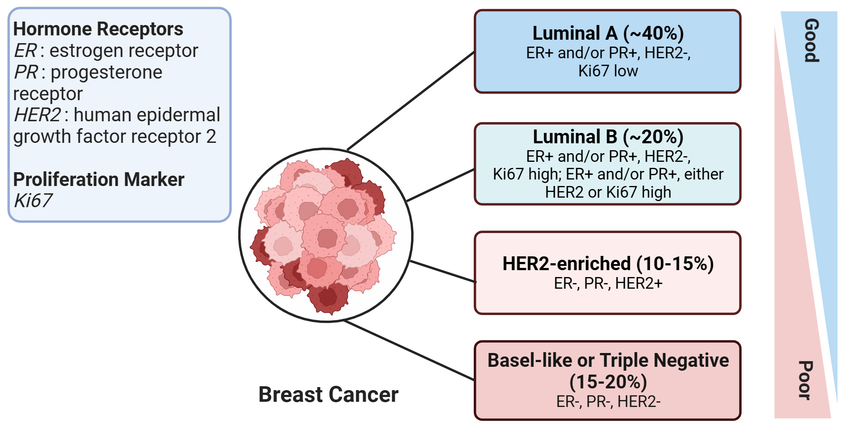
\includegraphics[width=0.8\linewidth]{reports/assets/subtypes.png}
	\caption{Los 4 subtipos moleculares del cáncer de mama y su porcentaje de relevancia \cite{harnessing_2024}}
	\label{fig:subtypes}
\end{figure}


En los últimos años, los avances en inteligencia artificial (IA), junto con la creciente disponibilidad de datos y una capacidad de cómputo cada vez más eficiente, han impulsado el desarrollo de modelos de aprendizaje profundo (DL) para tareas como la clasificación, detección y predicción del cáncer de mama, así como de otras enfermedades. Diversos estudios han demostrado que estos sistemas pueden igualar e incluso superar el desempeño de expertos humanos o sistemas CAD\footnote{Computer-Aided Diagnosis} en este tipo de tareas \cite{mckinney_international_2020,pattanaik_breast_2022,meenalochini_deep_2024,hussain_performance_2025}, lo que evidencia el impacto significativo de esta tecnología y su potencial beneficio para la práctica clínica y el bienestar de los pacientes.

Recientemente, se ha explorado la clasificación de subtipos moleculares a partir de imágenes mamográficas. Mota et al. (2024) \cite{mota_breast_2024} abordaron esta tarea, logrando un AUC del 60.62\% en clasificación multiclase con una arquitectura ResNet101. Por su parte, Rabah et al. (2025) \cite{ben_rabah_multimodal_2025} alcanzaron un AUC del 63.79\% aplicando un modelo Xception, y propusieron además un enfoque multimodal que integraba metadatos clínicos, elevando el rendimiento hasta un 88.87\% de AUC. Aunque los resultados obtenidos en escenarios unimodales son aún modestos y se encuentran por debajo del umbral de utilidad clínica establecido (\textasciitilde80\% AUC), estos estudios demuestran el potencial de la imagen como fuente diagnóstica y refuerzan la necesidad de continuar investigando en esta línea para mejorar la precisión y la utilidad clínica de estos modelos.

Este estudio propone un enfoque unimodal basado exclusivamente en mamografías del dataset público CMMD (The Chinese Mammography Database) \cite{cai_online_2023}, con el objetivo de comparar el rendimiento de arquitecturas Transformer de última generación como Vision Transformer (ViT), Shifted-Windows Transformer (SwinT) y Multi-Axis Vision Transformer (MaxViT), frente a un enfoque tradicional basado en redes convolucionales profundas (CNN). Aunque los modelos multimodales suelen lograr mejores resultados al integrar datos clínicos complementarios, centrarse únicamente en imágenes mamográficas presenta un alto valor práctico, especialmente en contextos con recursos limitados o donde la estandarización de los datos clínicos no está garantizada. Estudios recientes han evidenciado que los Transformers superan en precisión y robustez a las CNN en tareas de clasificación médica gracias a sus mecanismos de autoatención, que permiten capturar relaciones espaciales globales dentro de la imagen \cite{mauricio_comparing_2023}. Basándose en estas ventajas de diseño, este estudio plantea la hipótesis de que las arquitecturas Transformer podrían alcanzar un desempeño superior en la clasificación de subtipos moleculares, incluso bajo un enfoque unimodal.

En definitiva, este trabajo busca contribuir al desarrollo de herramientas diagnósticas no invasivas mediante la evaluación sistemática de modelos Transformer, con el fin de avanzar hacia una caracterización molecular automatizada, accesible y eficiente del cáncer de mama, especialmente en contextos donde la biopsia no es una opción inmediata, contribuyendo así a mejorar el acceso equitativo al diagnóstico y a reducir los tiempos de intervención terapéutica.

\section{Planificación}

\subsection{Definición de objetivos}

El \textbf{objetivo principal} de este estudio es explorar y evaluar el rendimiento de distintas arquitecturas de modelos del estado del arte basados en Transformers para la clasificación de subtipos moleculares del cáncer de mama a partir de mamografías, con el fin de contribuir al desarrollo de herramientas no invasivas que faciliten su caracterización. La premisa es que estos modelos se desempeñan mejor en tareas de clasificación y que sus mecanismos de atención podrían ayudar a capturar características relevantes que sirvan de apoyo para la caracterización tumoral.

Para alcanzar este objetivo, se plantean los siguientes \textbf{objetivos secundarios}:

\begin{enumerate}
	\item Revisar el estado del arte en la clasificación de subtipos moleculares mediante inteligencia artificial, identificando enfoques y resultados recientes.
	\item Implementar un pipeline de entrenamiento y evaluación, basado en validación cruzada, que permita estimar de forma robusta el rendimiento de modelos Transformer como ViT, SwinT y MaxViT.
	\item Analizar el impacto del desbalance de clases en el rendimiento de los modelos y aplicar técnicas de mitigación como el uso de funciones de pérdida ponderadas (\textit{weighted loss}), muestreo equilibrado (\textit{WeightedRandomSampler}) o aumentación de datos.
	\item Comparar los resultados obtenidos con un modelo convolucional de referencia (ResNet101), así como con estudios previos relevantes.
	\item Realizar un análisis estadístico que permita validar la significancia y la robustez de los resultados obtenidos.
	\item Aplicar técnicas de interpretabilidad como Grad-CAM o Attention Rollout sobre los modelos mejor desempeñados, para identificar regiones mamográficas asociadas a cada subtipo molecular.
	\item Interpretar y sintetizar los resultados obtenidos, proponiendo futuras mejoras y líneas de investigación alternativas.
\end{enumerate}


\subsection{Tareas a desarrollar}

\textbf{Estado del arte}

\begin{enumerate}
	\item Revisar la literatura científica actual sobre el cáncer de mama para contextualizar su relevancia clínica y epidemiológica.
	\item Analizar la importancia de la caracterización molecular del cáncer de mama, destacando sus ventajas, limitaciones y desafíos actuales.
	\item Examinar los avances recientes en el uso de inteligencia artificial y deep learning para la caracterización y diagnóstico del cáncer de mama, comparando enfoques y resultados reportados en la literatura.
\end{enumerate}

\textbf{Implementación}

\begin{enumerate}
	\item \textbf{Recolección de datos}: Obtención de las imágenes, conocer la estructura, organización y metadatos proporcionados por el dataset.
	\item \textbf{Análisis y preprocesamiento de datos}: Analizar la distribución de clases, coherencia de datos y realizar preprocesamiento de imágenes.
	\item \textbf{Codificación del proyecto}: Desarrollar el proyecto para llevar a cabo los experimentos, entrenamiento y evaluación de los diferentes modelos a evaluar.
	\item \textbf{Análisis de los resultados}: Comparar e interpretar los resultados obtenidos para plantear conclusiones y trabajos futuros.
\end{enumerate}

\textbf{Elaboración del reporte}

\begin{enumerate}
	\item \textbf{Escritura del reporte}: Escritura y documentación de los procedimientos llevados a cabo para realizar el proyecto, incluyendo metodología, materiales, resultados y conclusiones.
	\item \textbf{Correcciones}: Aplicar sugerencias ofrecidas por el tutor y refinar hasta alcanzar la calidad aceptada.
	\item \textbf{Entrega y presentación}: Entrega de la memoria y resumir los resultados más importantes para la presentación ante el comité.
\end{enumerate}

\subsection{Planificación}

A continuación, se presenta la planificación del proyecto, representada mediante un diagrama de Gantt que muestra las tareas previstas y su distribución temporal, que comprende 4 meses de trabajo divido en tareas de investigación, desarrollo y síntesis.

\begin{figure}[h!]
	\centering
	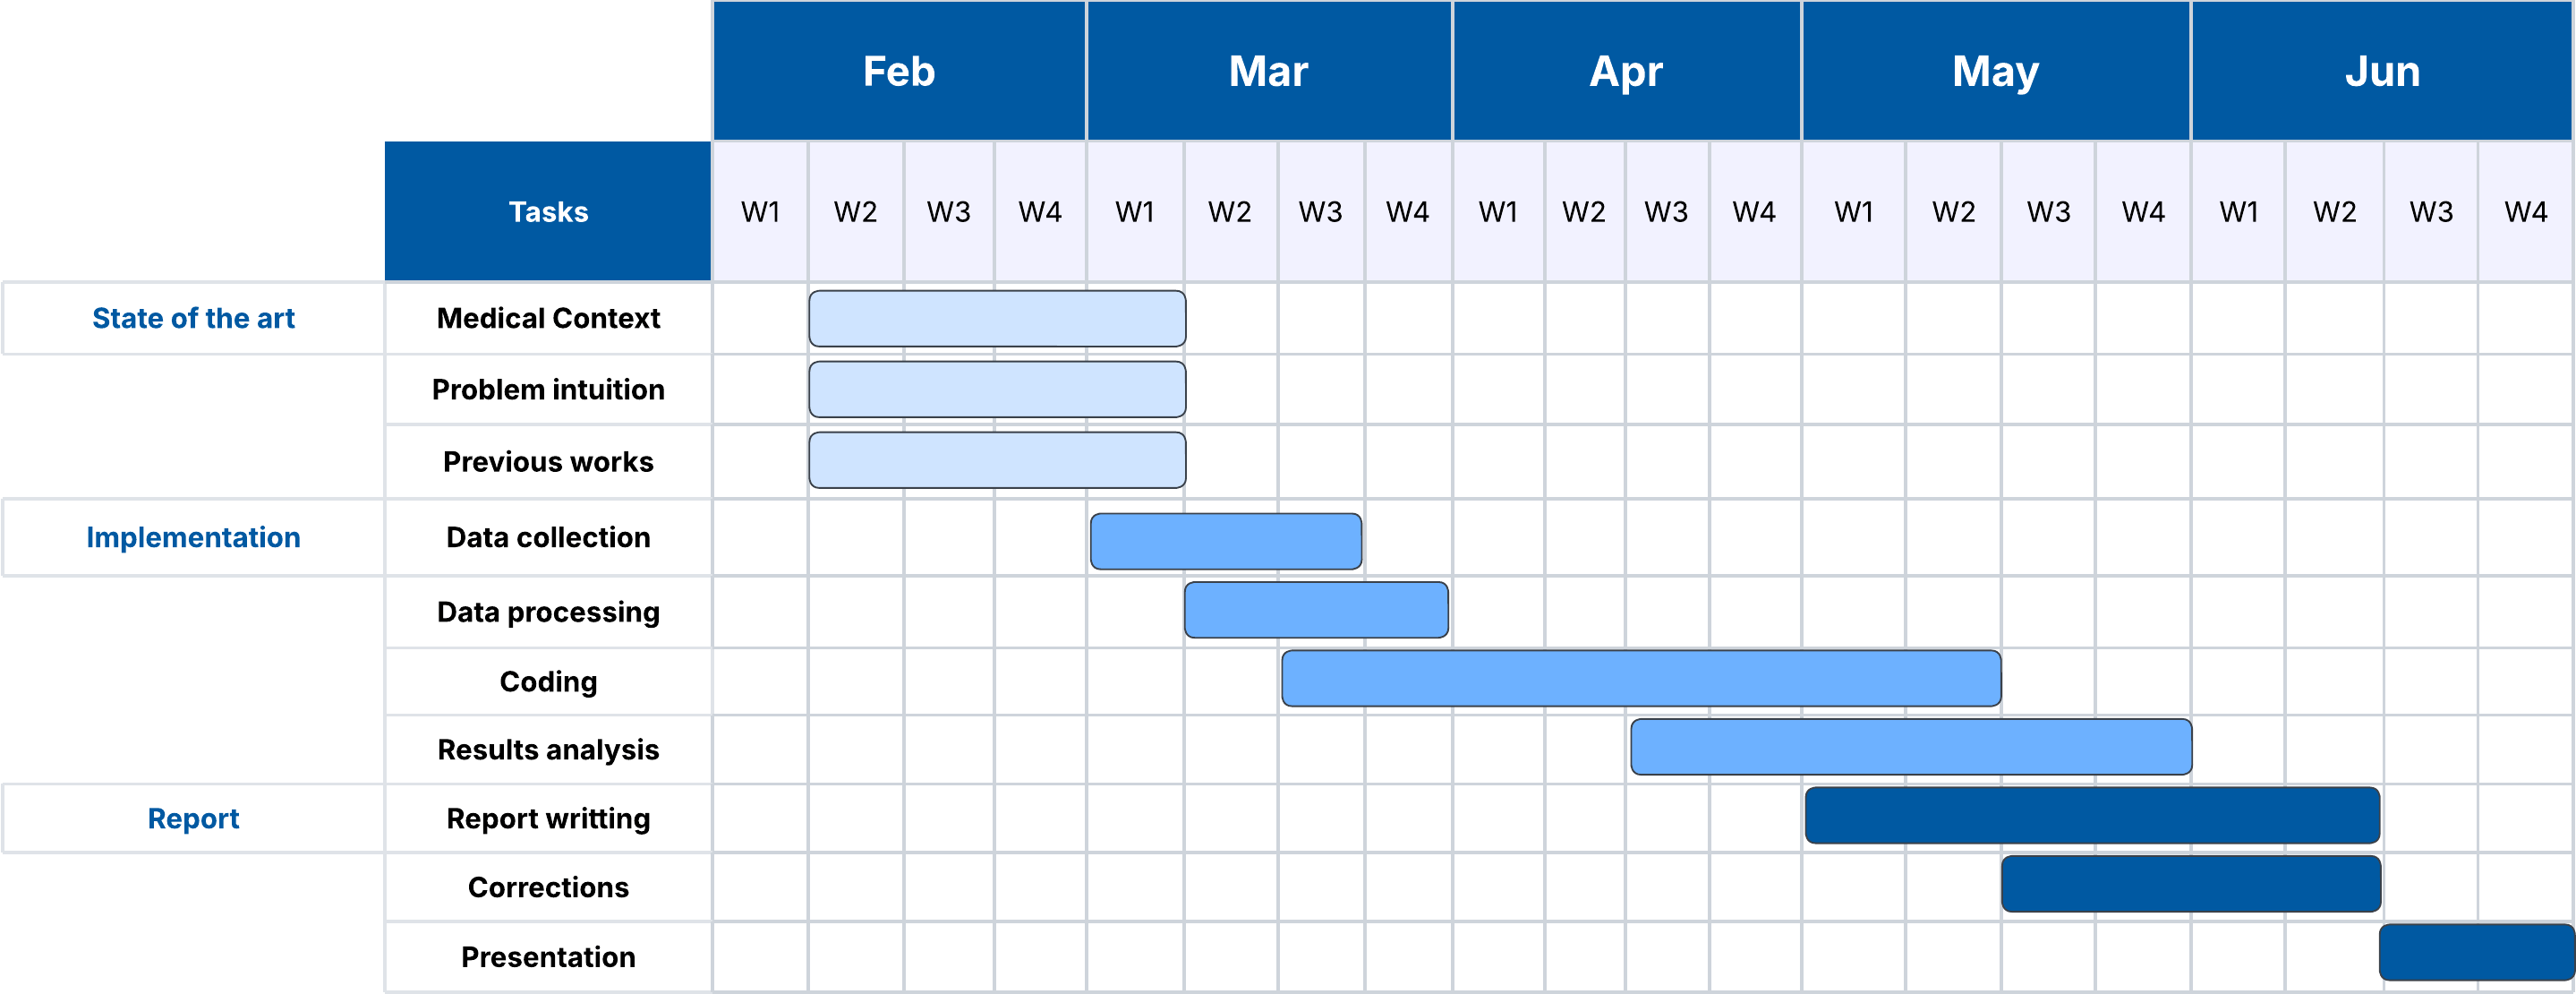
\includegraphics[width=1\linewidth]{reports//assets/RoadmapV3.png}
	\caption{Diagrama de Gantt}
	\label{fig:roadmap}
\end{figure}



%%%%%%%%%%%%%%%%%%%%%%%%%%%%%%%%%%%%%%%%%%%%%%%%%%%%%%%%%%%%%%%%%%%%%%%%%

\chapter{Antecedentes}

\section{Cáncer de mama}

El cáncer de mama es una neoplasia\footnote{Es un crecimiento anormal y descontrolado de células, que da lugar a una masa o tumor, se llama benigno si es de crecimiento lento y focalizado o maligno si es invasivo y rápido.} maligna que se origina en el tejido glandular de la mama, principalmente en los conductos y lobulillos, donde ciertas células sufren mutaciones genéticas que alteran su control de crecimiento celular. Estas alteraciones permiten que las células se multipliquen de manera descontrolada, formando masas tumorales que pueden infiltrar tejidos adyacentes y propagarse incluso a órganos distantes a través del sistema linfático y el torrente sanguíneo. En ausencia de un diagnóstico precoz y tratamiento oportuno, esta diseminación, también llamada metástasis, puede comprometer gravemente la supervivencia de la paciente.

\begin{figure}[h]
    \centering
    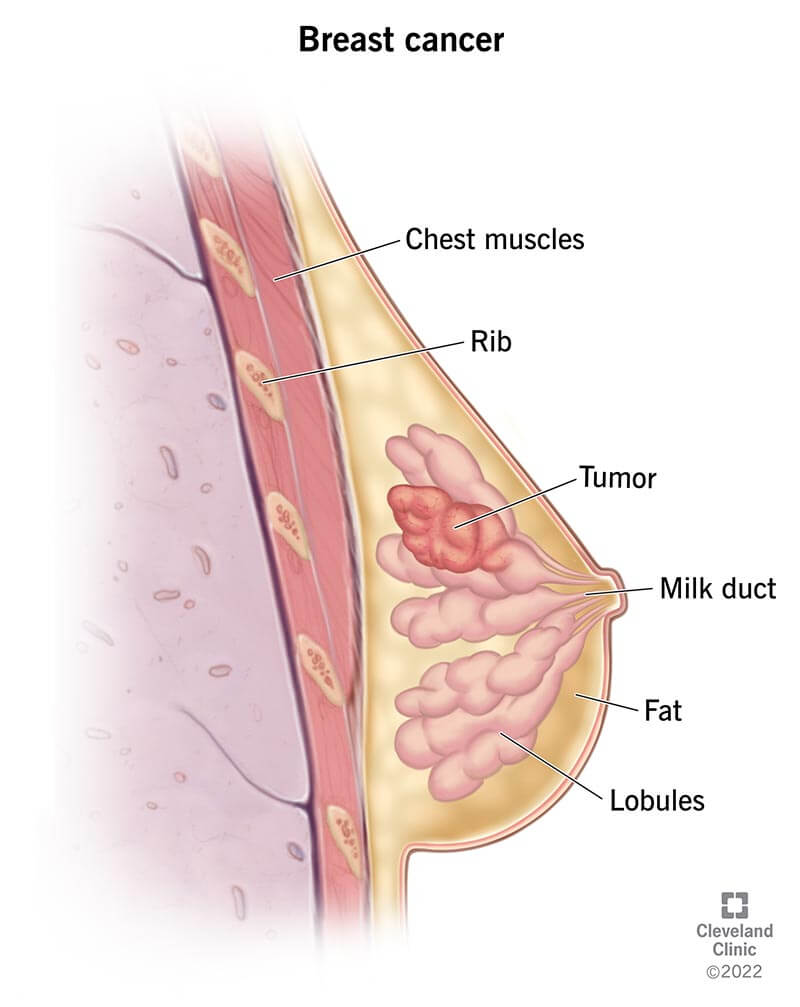
\includegraphics[width=0.3\linewidth]{reports//assets/bc.jpg}
    \caption{Anatomía del cáncer de mama \cite{cleveland_clinic_breast_2023}}
    \label{fig:breast-cancer-anatomy}
\end{figure}

\subsection{Epidemiología}

A nivel mundial, es la neoplasia más frecuente entre mujeres y es la principal causa de mortalidad oncológica en esta población. En 2022, se estimaron aproximadamente 2.3 millones de nuevos casos y se registraron 670.000 muertes por esta enfermedad, según datos de la Organización Mundial de la Salud (OMS) \cite{who_breast_2024}. En España, representa casi el 30\% de todos los casos de cáncer y se estima que en 2025 se registren aproximadamente 37,400 nuevos casos, según las proyecciones y estudios de la Asociación Española de Oncología Médica (SEOM) \cite{seom_cancer_nodate}.

\subsection{Clasificación clínica}

La mayoría de los cánceres de mama son carcinomas, es decir, tumores malignos que se originan en los conductos o lóbulos mamarios. Desde una perspectiva clínica, estos tumores se pueden clasificar según diferentes criterios, entre los que destacan:

\textbf{Según su grado de invasión}
\begin{itemize}
    \item \textbf{Carcinoma in situ}: Se trata de un tumor en el que las células anormales están solo dentro de los conductos de la mama y no han atravesado la barrera natural que los separa del resto del tejido mamario. Aunque no es invasivo, se considera una lesión precursora y de alto riesgo.
    \item \textbf{Carcinoma invasivo}: Es un tumor que ha atravesado los conductos o lobulillos de la mama y ha invadido el tejido mamario que los rodea. Puede diseminarse a ganglios linfáticos o a distancia.
\end{itemize}

\textbf{Según su origen histológico}
\begin{itemize}

    \item \textbf{Carcinoma ductal}: Se origina en los conductos galactóforos\footnote{Conductos que transportan la leche desde las glándulas mamarias hasta el pezón.} y es el subtipo más común.
    \item \textbf{Carcinoma lobulillar}: Se origina en los lóbulos mamarios y suele presentar un patrón de diseminación más difuso.
\end{itemize}

\textbf{Según hallazgos radiológicos}

La clasificación radiológica se basa en las características observadas mediante mamografía, ecografía o resonancia magnética. El sistema BI-RADS (Breast Imaging-Reporting and Data System) permite estandarizar la interpretación y asignar una categoría de sospecha que guía la conducta médica (seguimiento, biopsia, etc.).

En las figuras \ref{fig:histological_types_one} y \ref{fig:histological_types_two} se observan las diferencias entre carcinoma ductal y lobulillar tanto in situ como invasivo.

\begin{figure}[h!]
    \centering
    \begin{subfigure}[c]{0.48\textwidth}
        \centering
        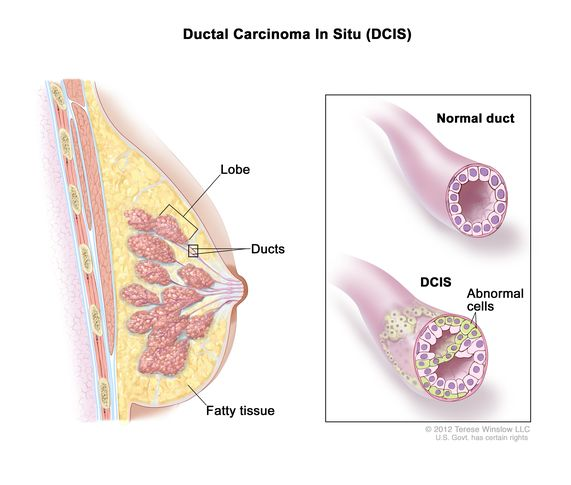
\includegraphics[width=\textwidth]{reports/assets/dcis.jpg}
        \caption{Carcinoma ductal in situ}
        \label{fig:dcis}
    \end{subfigure}
    \begin{subfigure}[c]{0.48\textwidth}
        \centering
        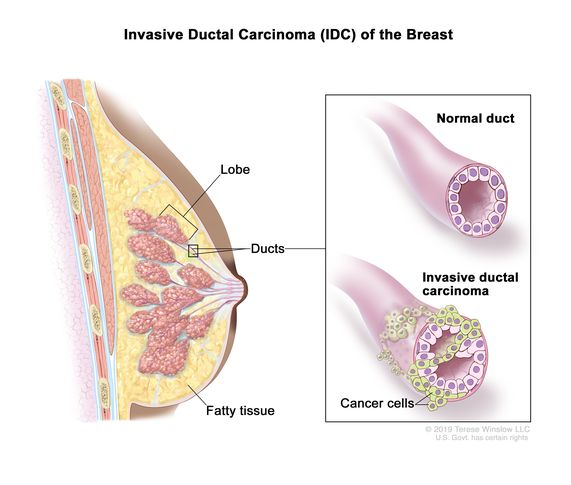
\includegraphics[width=\textwidth]{reports/assets/idc.jpg}
        \caption{Carcinoma ductal invasivo}
        \label{fig:idc}
    \end{subfigure}
    \caption{Ductal in situ vs. invasivo \cite{noauthor_nci_2011}}
    \label{fig:histological_types_one}
\end{figure}

\begin{figure}[h!]
    \centering
    \begin{subfigure}[c]{0.48\textwidth}
        \centering
        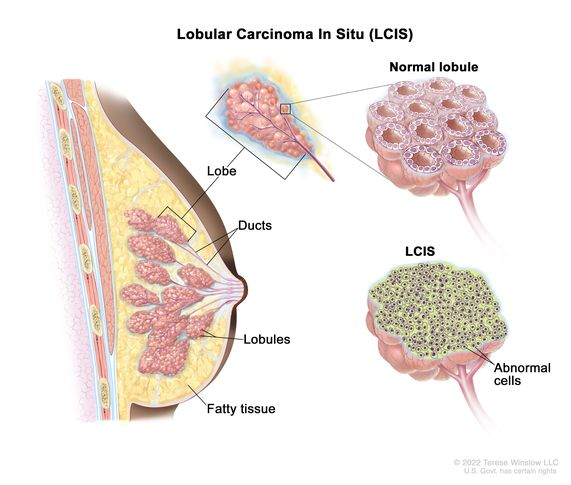
\includegraphics[width=\textwidth]{reports/assets/lcis.jpg}
        \caption{Carcinoma lobulillar in situ}
        \label{fig:lcis}
    \end{subfigure}
    \begin{subfigure}[c]{0.48\textwidth}
        \centering
        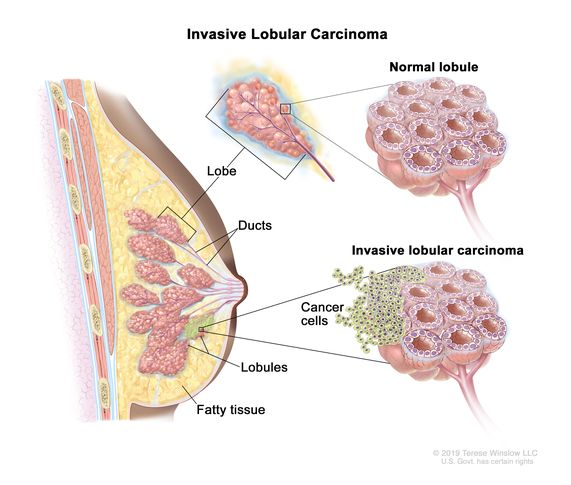
\includegraphics[width=\textwidth]{reports/assets/ilc.jpg}
        \caption{Carcinoma lobulillar invasivo}
        \label{fig:ilc}
    \end{subfigure}
    \caption{Lobulillar in situ vs. invasivo \cite{noauthor_nci_2011}}
    \label{fig:histological_types_two}
\end{figure}

Además de estas clasificaciones, en los últimos años ha adquirido especial relevancia la tipificación molecular del cáncer de mama, basada en la expresión de biomarcadores y perfiles genómicos, la cual será abordada en la siguiente sección.


\subsection{Subtipos moleculares}

Aunque la clasificación clínica e histológica del cáncer de mama proporciona información relevante para el diagnóstico, no siempre permite predecir con precisión el comportamiento biológico del tumor ni su respuesta a tratamientos específicos. 

Fueron las investigaciones de Perou et al. (2000) \cite{perou_molecular_2000} y Sørli et al. (2003) \cite{sorlie_repeated_2003} las que sentaron las bases para la caracterización molecular del cáncer de mama. Mediante el análisis de perfiles de expresión génica\footnote{Estudio que permite identificar qué genes están activos y en que cantidad en una célula o tejido, analizando los niveles de ARN producidos por miles de genes simultáneamente.}, Perou et al. demostraron que el cáncer de mama es una enfermedad heterogénea y propusieron una clasificación en subtipos moleculares que se basó en los patrones de expresión genética de los tumores analizados. Así se definieron inicialmente cuatro subtipos, \textbf{Luminal A}, \textbf{Luminal B}, \textbf{HER2}, \textbf{Basal-like (Triple negativo)}.

Por su parte, Sørli et al. reforzaron estos hallazgos. Reprodujeron la investigación en diferentes cohortes de pacientes, demostrando que los hallazgos no eran artefactos de un solo estudio. Además, demostraron que los subtipos moleculares se asocian con diferencias clínicamente significativas, como el pronóstico y riesgo de metástasis a distancia, lo cual proporcionó a esta caracterización un valor predictivo superior a la clasificación histológica tradicional.

\begin{figure}
    \centering
    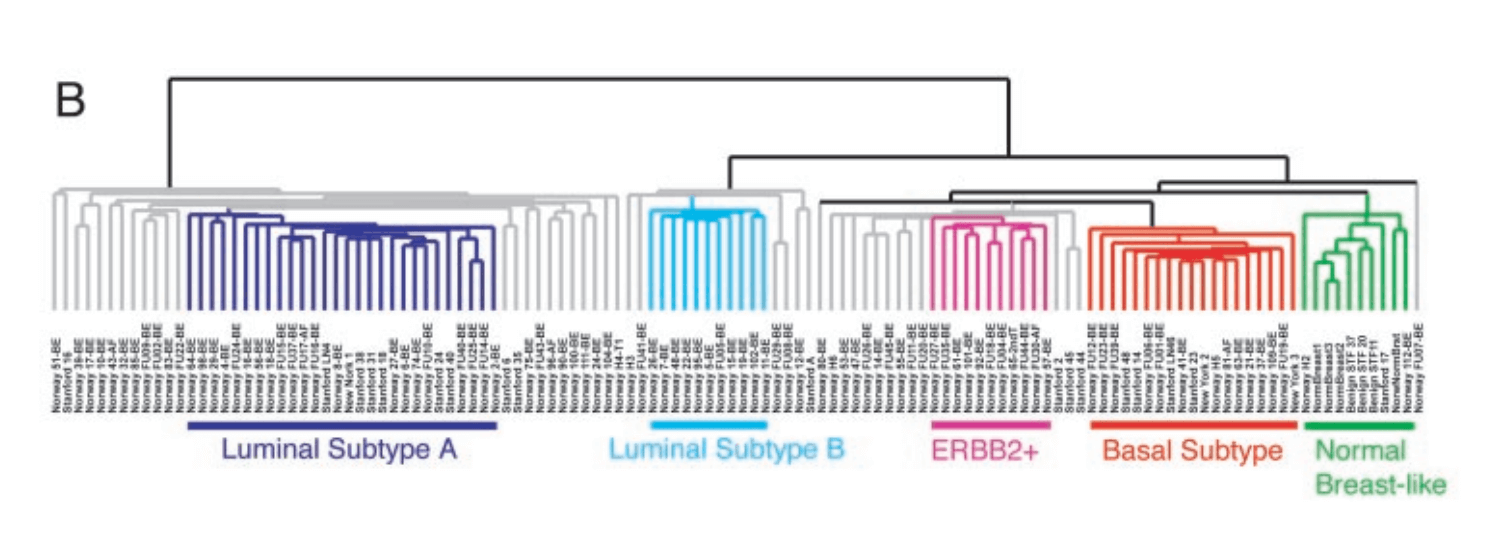
\includegraphics[width=0.8\linewidth]{reports//assets/dendogram.png}
    \caption{Dendrograma del estudio de Sørli et al. que muestra el agrupamiento de subtipos según los patrones genéticos \cite{sorlie_repeated_2003}.}
    \label{fig:sorlie-dandrogram}
\end{figure}


A partir de estos estudios, los esfuerzos se centraron en llevar los resultados a la práctica clínica. Debido a que la técnica utilizada para la clasificación en ese momento (microarrays de ADN) era costosa, compleja y no accesible para la mayoría de centros hospitalarios, se buscó una alternativa. Fue en los consensos internacionales de St. Gallen donde se propusieron criterios de clasificación basados en marcadores inmunohistoquímicos (IHQ) y se formalizan los subtipos utilizando una combinación de los siguientes receptores hormonales \cite{lips_breast_2013}:

\begin{itemize}
    \item \textbf{Receptores de Estrógeno (RE) y Progesterona (RP)}: Definen la dependencia hormonal del tumor que puede afectar su crecimiento. Responden bien a terapia hormonal.
    \item \textbf{HER2 (Human epidermal growth factor receptor 2)}: Proteína que estimula el crecimiento celular. Su sobreexpresión suele indicar un subtipo más agresivo.
    \item \textbf{Ki-67}: Es el índice de proliferación celular. Un Ki-67 alto sugiere un tumor con mayor agresividad y rápida proliferación.
\end{itemize}

\begin{table}
    \centering
    \begin{tabular}{lccccc}
        \toprule
        \textbf{Subtipo} & \textbf{HER2} & \textbf{ER} & \textbf{PR} & \textbf{Ki-67} \\
        \midrule
        Luminal A & Negativo & Positivo & Positivo & < 14\% \\
        Luminal B/HER2- & Negativo & Positivo & - & $\geq$ 14\% \\
        Luminal B/HER2+ & Positivo & Positivo & - & - \\
        HER2-enriched & Positive & Negativo & Negativo & - \\
        Triple Negativo & Negativo & Negativo & Negativo & - \\
        \bottomrule
    \end{tabular}
    \caption{Criterios de clasificación de subtipos moleculares del consenso de St. Gallen 2013 \cite{goldhirsch_personalizing_2013}}.
    \label{tab:molecular_subtypes_comb}
\end{table}

En el cuadro \ref{tab:molecular_subtypes_comb} se pueden observar dichos criterios de clasificación.

El subtipo Luminal A es el más frecuente, representando 70\% de las muestras al momento del diagnóstico. Se caracterizan por un crecimiento más lento y responden bien a las terapias hormonales, lo que los convierte en tumores de mejor pronóstico y mayores posibilidades de supervivencia. Los del grupo Luminal B son más agresivos y, por tanto, con un pronóstico más reservado y con más probabilidades de recurrencia, suelen resistirse más a los tratamientos hormonales y pueden necesitar quimioterapia. 

Por su parte, los tumores HER2-enriched representan entre el 10\% y el 15\% de los casos, y se distinguen por una rápida tasa de crecimiento y por la sobreexpresión del receptor HER2, sin presencia de receptores hormonales y finalmente, el subtipo triple negativo, que también aparece en un 10–15\% de los diagnósticos, carece de expresión de RE, RP y HER2. Este grupo presenta un comportamiento clínico más agresivo, con alta tasa de recaídas tempranas y una limitada gama de opciones terapéuticas, ya que no responde a la hormonoterapia ni a los tratamientos dirigidos. La quimioterapia convencional es actualmente la principal estrategia terapéutica.

\section{Imagen médica}

La imagen médica representa un conjunto de técnicas y procedimientos utilizados para generar representaciones visuales del interior del cuerpo humano con fines clínicos y científicos. Estas herramientas permiten la visualización no invasiva de estructuras anatómicas y procesos fisiológicos, facilitando tanto el diagnóstico de enfermedades como el estudio de la anatomía física y metabólica.

\section{Cribado del cáncer}
\section{Inteligencia artificial en la imagen médica}
\section{Clasificación de subtipos moleculares mediante imagen}

\chapter{Revisión tecnológica}

En este apartado se exploran las definiciones y estructuras modernas de modelos de inteligencia artificial, así como también su uso en medicina moderna y en específico en imagen médica.


\section{Inteligencia artificial}
\subsection{De la IA clásica al Deep Learning}
\subsection{Línea de tiempo}

\section{Redes neuronales convolucionales}
\subsection{Principios generales}
\subsection{Arquitecturas y variantes históricas}
\subsection{Limitaciones en mamografía}


\section{Transformers para visión}
\subsection{Breve historia}
\subsection{Principios de la autoatención}
\subsection{Vision Transformer (ViT)}
\subsection{Shifted-Window Transformer (Swin)}
\subsection{Multi-Axis Vision Transformer (MaxViT)}
\section{Técnicas de entrenamiento y evaluación}
\subsection{Transfer learning y fine-tuning}
\subsection{Validación cruzada K-Fold}



\chapter{Materiales y metodología}

En esta sección se documentan los materiales y procesos llevados a cabo para la realización de este estudio. Se describe en primer lugar el conjunto de datos seleccionado para el entrenamiento y análisis de los modelos, seguido del procesamiento y preparación de las imágenes, y finalmente las métricas de evaluación empleadas para valorar el rendimiento de los modelos.

\section{The Chinese Mammography Database}

El Chinese Mammography Database (CMMD) es un conjunto de datos público, desarrollado por Cai et al. (2023) \cite{cai_online_2023} y alojado en The Cancer Imaging Archive (TCIA)\footnote{\url{https://www.cancerimagingarchive.net/collection/cmmd/}}. Este dataset incluye un total de 3.712 mamografías correspondientes a 1.775 pacientes de origen chino, en vistas cráneo-caudal (CC) y medio-lateral oblicua (MLO), recolectadas entre julio de 2012 y enero de 2016. El CMMD se divide en dos subconjuntos: CMMD1, que contiene estudios con información clínica básica, y CMMD2, que incluye además anotaciones del subtipo molecular. Este último constituye la base principal de la presente investigación, al ser el único subconjunto público y de libre acceso que proporciona dichas etiquetas moleculares de forma explícita.

En el cuadro \ref{tab:cmmd_features} se detallan las características principales de cada subconjunto.


\begin{table}
    \centering
    \begin{tabular}{lccccc}
        \toprule
        & \textbf{CMMD1} & \textbf{CMMD2} & \\
        \midrule
        \textbf{Número de pacientes} & 1026 & 749 & 1775\\
        \textbf{Número de imágenes} & 2214 & 1498 & 3712\\
        \textbf{Edad media de pacientes} & 45.92 (17-84 años) & 49.82 (21-87 años) & - \\
        \textbf{Categorías} & Benigno y Maligno & Solo maligno & - \\
        \textbf{Subtipo molecular} & No & Si & - \\
        \bottomrule
    \end{tabular}
    \caption{Características de los subconjuntos del CMMD}
    \label{tab:cmmd_features}
\end{table}


\subsection{Descripción general y análisis}

Como se ha mencionado anteriormente, para la realización de estudio, el enfoque estará en el subconjunto de CMMD2. Para la conformación del mismo, se seleccionaron únicamente los casos malignos con información completa de los marcadores inmunohistoquímicos y diagnóstico de carcinoma invasivo, tal como se detalla en los criterios de exclusión representados en la Figura \ref{fig:cmmd_criteria}. Tras aplicar estos criterios, la muestra final quedó constituida por 1,498 imágenes correspondientes a 749 pacientes.


\begin{figure}[h]
	\centering
	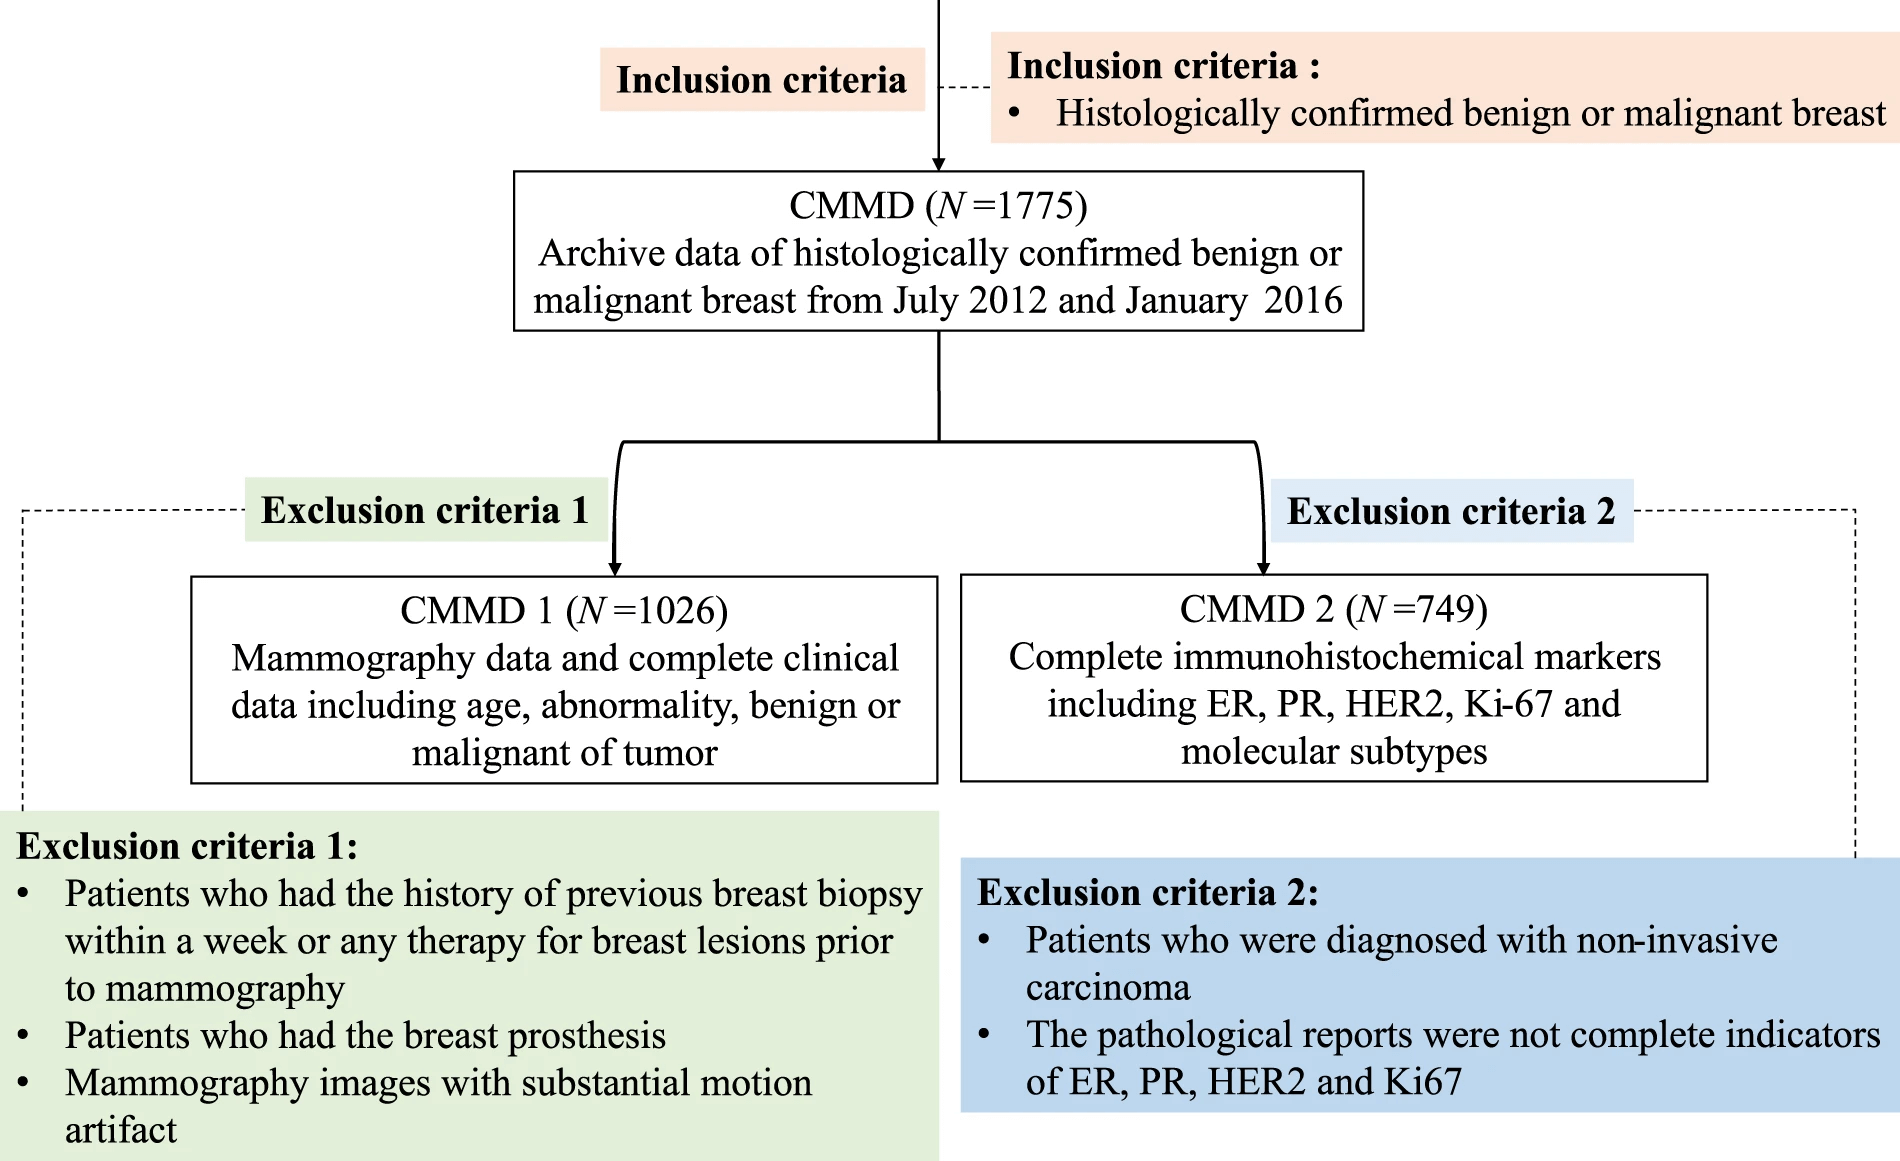
\includegraphics[width=0.8\linewidth]{reports//assets/cmmd_criteria.png}
	\caption{Criterios de exclusión del CMMD \cite{cai_online_2023}}
	\label{fig:cmmd_criteria}
\end{figure}


\textbf{Recolección de las imágenes}

Las imágenes fueron recolectadas mediante el uso del sistema de mamografía \textbf{GE Senographe DS}, obteniendo por cada paciente tanto la vista cráneo-caudal como la medio-lateral oblicua, esto representa una limitación del conjunto de datos que se explorará más adelante. Posteriormente, fueron almacenadas en escala de grises de 8-bits y en una resolución de 2294x1914 píxeles \cite{cai_online_2023}.

\textbf{Formato y resolución de las imágenes}

El formato principal de las imágenes del conjunto de datos es DICOM (Digital Imaging and Communications in Medicine), el estándar en imagen médica, ya que permite almacenar metadatos clínicos junto con la imagen y permite la interoperabilidad entre equipos de diferentes fabricantes así como también la interacción entre diferentes sistemas informáticos en hospitales y centros de salud.

\textbf{Metadatos}

Para cada paciente, el conjunto de datos proporciona un fichero CSV (Comma Separated Values)\footnote{Archivo de texto plano que almacena datos en forma de tabla, donde cada línea representa una fila y cada valor de la fila está separado por una coma} con información adicional a las imágenes obtenidas, incluyendo la edad, la lateralidad, el tipo de anormalidad, la clasificación  y, en el caso del CMMD2, también el subtipo molecular al que pertenece el tumor. La Tabla \ref{tab:cmmd2_metadata} describe en detalle estos datos.


\begin{table}[h]
    \centering
    \begin{tabular}{>{\bfseries}l p{5cm} p{6cm}}
        \toprule
        \textbf{Columna} & \textbf{Descripción} & \textbf{Valores posibles} \\
        \midrule
        ID1 & Identificador único del paciente & Formato: D2-XXXX \\
        LeftRight & Lateralidad de la mama & L (izquierda), R (derecha) \\
        Age & Edad del paciente al momento del estudio & Entre 21 y 87 años \\
        Number & Número de imágenes disponibles por estudio & Entre 2 y 4 \\
        Abnormality & Tipo de anomalía & Masa, Calcificación, Ambas \\
        Classification & Naturaleza de la anomalía & Benigna, Maligna \\
        Subtype & Subtipo molecular del cáncer de mama & Luminal A, Luminal B, HER2-enriquecido, Triple negativo \\
        \bottomrule
    \end{tabular}
    \caption{Descripción de las variables presentes en los metadatos del conjunto CMMD.}
    \label{tab:cmmd2_metadata}
\end{table}

Es importante destacar que, en el caso del CMMD2, la columna lateralidad indica el lado donde fue encontrado el tumor, por tanto, el lado contrario se considera benigno \cite{cai_online_2023}.

La distribución de la edad de las pacientes sigue aproximadamente una distribución normal, aunque presenta ligeras asimetrías. El rango de edad más frecuente se sitúa entre los 45 y 55 años, lo cual es coherente con la epidemiología del cáncer de mama, ya que la mayoría de los casos se detectan en ese intervalo. La inclusión de pacientes jóvenes en el conjunto de datos también aporta diversidad y permite analizar el comportamiento de los modelos en subpoblaciones menos representadas.

\begin{figure}[h!]
    \centering
    \begin{subfigure}[c]{0.49\textwidth}
        \centering
        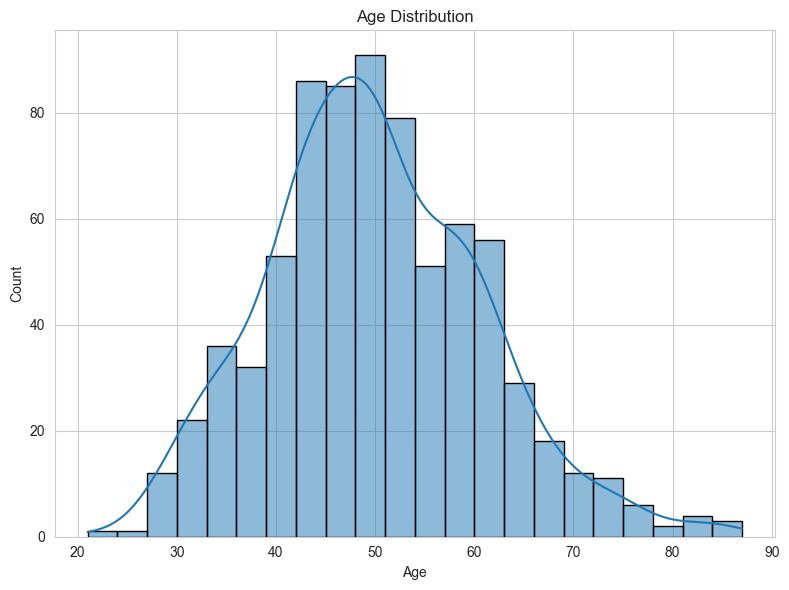
\includegraphics[width=\textwidth]{reports//assets/age.png}
        \caption{Distribución por edad}
        \label{fig:age_dist}
    \end{subfigure}
    \begin{subfigure}[c]{0.49\textwidth}
        \centering
        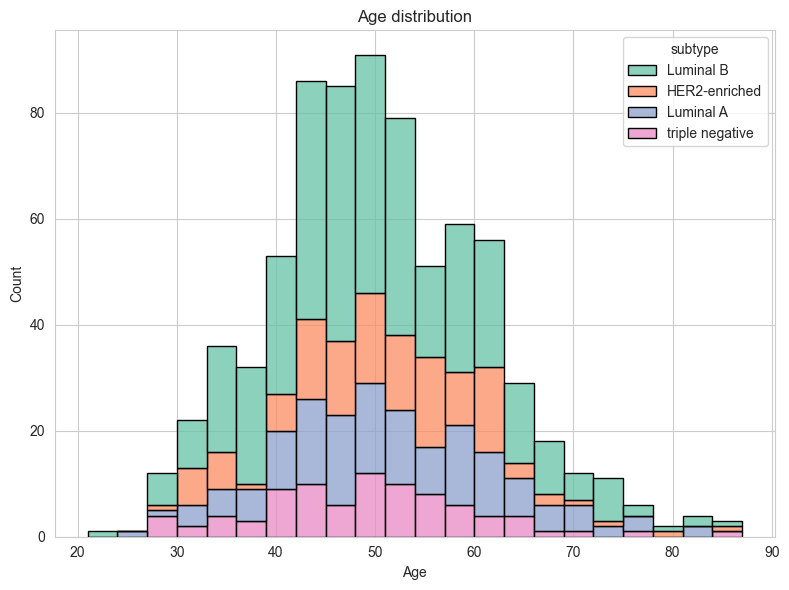
\includegraphics[width=\textwidth]{reports/assets/age_subtype.png}
        \caption{Distribución por edad y subtipo}
        \label{fig:age_subtype}
    \end{subfigure}
    \caption{Distribución por edad de los pacientes (CMMD2)}
    \label{fig:age_dist_all}
\end{figure}

En la Figura \ref{fig:age_dist_all} podemos observar dicha distribución, así como también una vista a la distribución de los subtipos presentados.

Por otro lado, analizar la distribución de los subtipos moleculares en el conjunto CMMD2 es un aspecto crucial, ya que determina la representatividad estadística de cada clase y, por ende, la capacidad de los modelos para generalizar adecuadamente en escenarios clínicos reales. En este conjunto se observa un fuerte desbalance de clases\footnote{Se habla de desbalance cuando una o más clases están representadas con una frecuencia significativamente mayor o menor que el resto.}, siendo el subtipo Luminal A el más prevalente, con 376 pacientes, seguido por Luminal B con 152 casos y HER2-enriquecido con 135. Finalmente, el subtipo Triple Negativo es el menos representado, con apenas 86 pacientes.

Esta desproporción también se refleja en el número de imágenes disponibles por clase, ya que cada paciente cuenta con al menos dos imágenes (proyecciones CC y MLO), salvo en algunos casos excepcionales, además esta desigualdad plantea un desafío importante para los modelos de clasificación, que tienden a favorecer las clases mayoritarias si no se aplican estrategias de compensación adecuadas. Sin embargo, refleja con fidelidad la prevalencia relativa observada en la práctica clínica, donde los subtipos Luminales son los más frecuentes y los casos Triple Negativo representan una proporción menor.

\begin{figure}[h!]
    \centering
    \begin{subfigure}[c]{0.45\textwidth}
        \centering
        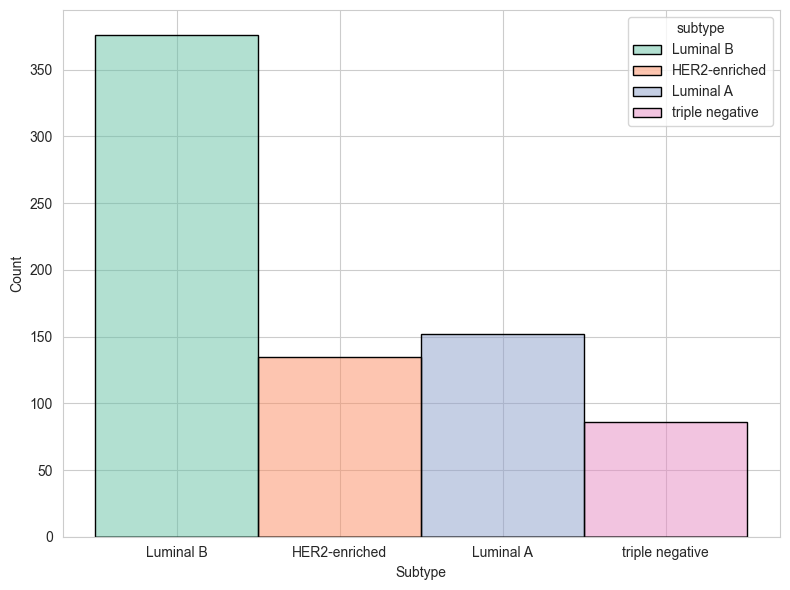
\includegraphics[width=\textwidth]{reports//assets/subtype_hist.png}
        \caption{Distribución por edad}
        \label{fig:subtype_hist}
    \end{subfigure}
    \begin{subfigure}[c]{0.45\textwidth}
        \centering
        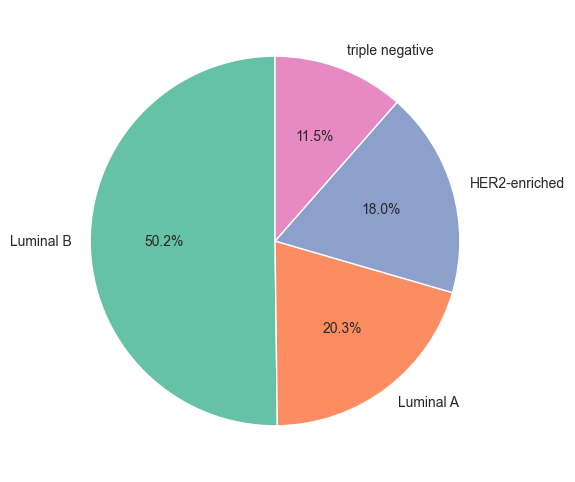
\includegraphics[width=\textwidth]{reports/assets/subtype_pie.png}
        \caption{Distribución por edad y subtipo}
        \label{fig:subtype_pie}
    \end{subfigure}
    \caption{Distribución por edad de los pacientes (CMMD2)}
    \label{fig:subtype_charts}
\end{figure}


\begin{figure}
    \centering
    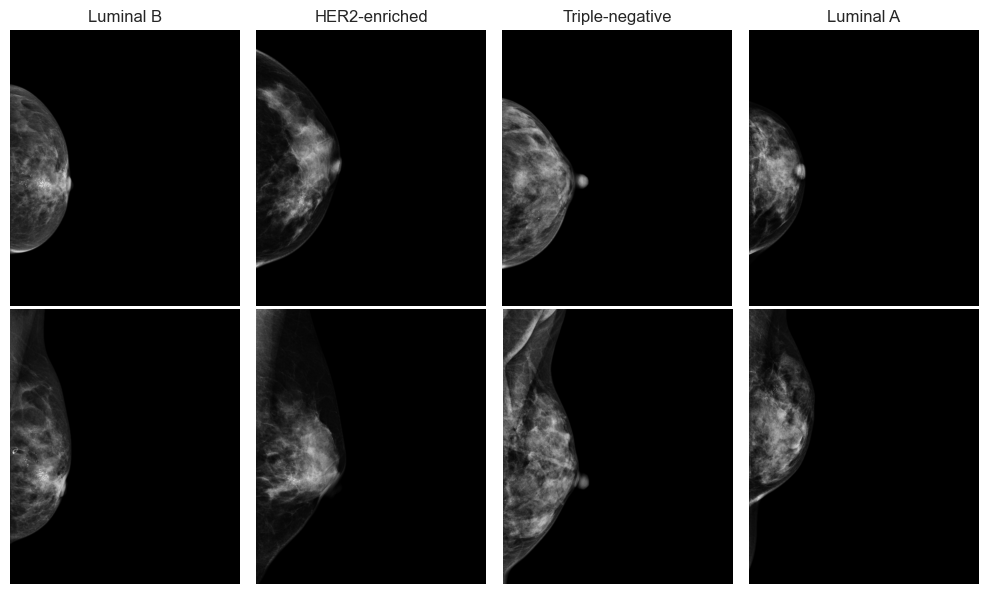
\includegraphics[width=1\linewidth]{reports//assets/images_examples.png}
    \caption{Ilustración de dos ejemplos por cada subtipo molecular (CC y MLO)}
    \label{fig:cmmd-examples}
\end{figure}

\section{La revisión TOMPEI-CMMD}
\section{Preprocesamiento de imágenes}
\section{Partición y estratificación de datos}
\section{Métricas de evaluación}


\chapter{Resultados y discusión}
\section{Resultados}

\chapter{Conclusiones y trabajo futuro}

%%%%%%%%%%%%%%%%%%%%%%%%%%%%%%%%%%%%%%%%%%%%%%%%%%%%%%%%%%%%%%%%%%%%%%%%%
\backmatter
\selectlanguage{spanish}
\addcontentsline{toc}{chapter}{Bibliografía}
\bibliographystyle{IEEEtran}
\bibliography{references}


\end{document}